% File: chapters/discussion.tex

\chapter{Discussion and Conclusion}
\label{chap:discussion}

This chapter interprets the experimental results from Chapter 5, connects them to the research questions posed in Chapter 1, and examines what the findings mean for practitioners. We discuss both successes and failures, then close with recommendations for future research and a summary of contributions.


\section{Interpretation of Results}
\label{sec:discussion_interpretation}

\subsection{What the Data Reveals}
\label{sec:discussion_data}

The experimental results revealed patterns we did not anticipate at the outset of this work.

Most surprising was the inverse relationship between model size and performance. Conventional wisdom in machine learning suggests larger models perform better. Our fuzz driver experiments showed something different.

Why did the larger general-purpose models fail while smaller specialized ones succeeded? We analyzed the generated code outputs and identified a consistent pattern. The larger models generated code that appeared syntactically plausible but did not align with the structural requirements of the fuzz driver task. They would create elaborate test scaffolding, call APIs in reasonable sequences, but miss the essential structure that a libFuzzer driver requires. The \texttt{LLVMFuzzerTestOneInput} function signature was wrong. The input parsing was incorrect.

Qwen 2.5-Coder succeeded because it was trained specifically on code generation tasks. It understood the structural patterns of fuzz drivers from its training data. The model had seen enough examples of the correct form to reproduce it reliably. This matters more than raw parameter count.

The LoRA fine-tuning results reinforced this insight. A small 1.5 billion parameter model, after adaptation on high-quality OSS-Fuzz drivers, produced outputs matching the quality of much larger models while using markedly fewer resources. Specialized knowledge compensated for reduced parameter count.

These findings challenge a common assumption in AI deployment. Organizations often select the largest model available, assuming a higher parameter count correlates with better results. Our data suggests this does not hold for specialized code generation tasks. A well-chosen smaller model, possibly with domain-specific fine-tuning, can match or exceed larger alternatives at a fraction of the cost.

What about the coverage numbers? The original thesis proposal considered that achieving even 40\% coverage while saving hours of expert time would constitute meaningful progress. By this standard, the automated approach succeeded. However, as discussed in Chapter 5, our examination of comparable manually-written fuzz drivers in OSS-Fuzz projects suggests expert-crafted drivers typically achieve 60 to 80\% line coverage for similar libraries, because they incorporate domain knowledge about edge cases that LLMs may miss.

This gap matters, but so does the time investment. A skilled security engineer might spend 2 to 8 hours writing and debugging a fuzz driver for a new library. Our automated pipeline generates a usable driver in approximately 30 minutes. Even if the automated driver achieves lower coverage, the time savings are meaningful.


\subsection{Unexpected Findings: Network Architecture}
\label{sec:discussion_network}

We anticipated the core technical challenge would be generating high-quality fuzz drivers. We expected difficulties with C++ complexity, API understanding, or coverage optimization. We planned our research around these expected challenges.

Infrastructure integration constituted a major focus of the implementation effort.

When we moved from local experiments to CARIAD's production environment, we identified that integrating with the corporate network architecture required additional design considerations. The CI/CD runners operated in isolated network segments by design, and external API access required explicit network path configuration. Our architecture assumed we could call LLM services from build processes, but the corporate network security policies required a tailored approach.

Resolving this required evaluating several architectural approaches. The existing proxy infrastructure was configured for approved HTTP destinations, and the runner environment was designed without VPN client capabilities, consistent with its security-hardened configuration. Caching model responses was considered but would not support dynamic code generation effectively.

We collaborated with CARIAD's infrastructure team to provision Azure Private Link endpoints. This technology creates a private connection between the corporate network and Azure services, appearing as an internal address rather than external internet. The LLM API becomes reachable without traversing the public internet.

The architecture of this solution is illustrated in Figure~\ref{fig:enterprise_network}, which shows how the Azure Private Link creates a secure tunnel between the CARIAD internal network and Azure OpenAI services, routing traffic through a private connection rather than the public internet while maintaining security compliance.

\begin{figure}[htbp]
\centering
\caption{Enterprise Network Architecture with Azure Private Link}
\label{fig:enterprise_network}
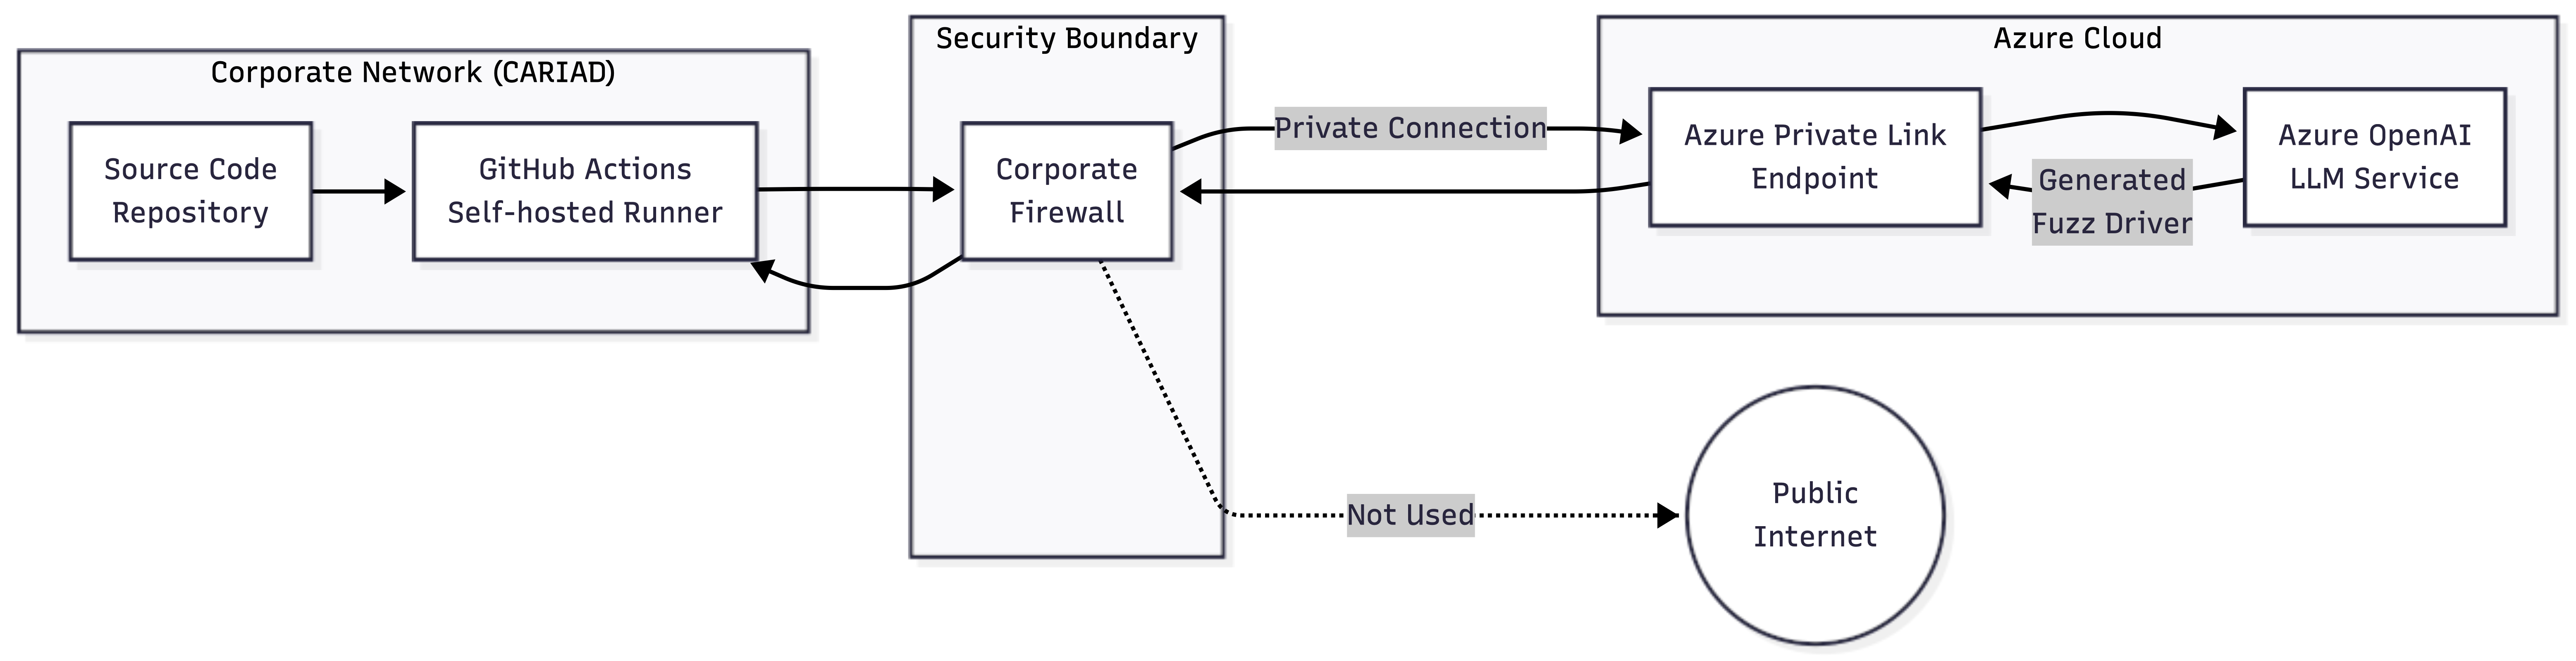
\includegraphics[width=\linewidth]{bilder/figure6_1_network_architecture.png}
\end{figure}

Setting up Private Link involved organizational coordination, including approval processes, security reviews, configuration testing, and documentation, which are standard steps for enterprise deployments in regulated industries. The technical configuration itself was manageable once approvals were obtained, requiring approximately one month from initial request to operational deployment.

This experience provided an important insight about AI deployment in enterprise environments. The machine learning components are complemented by infrastructure integration requirements. Enterprise environments introduce additional considerations, including network architecture, security compliance, and provisioning workflows, that differ from academic research settings. Anyone planning to deploy LLM-based tools in large organizations should allocate appropriate time for enterprise integration alongside the technical implementation. Based on our experience, organizations should plan for a 2- to 3-month enterprise integration timeline to accommodate standard provisioning and compliance workflows.


\section{Addressing Research Questions}
\label{sec:discussion_rq}

\subsection{Primary Research Question Analysis}
\label{sec:discussion_rq_primary}

\textbf{RQ1: Can Large Language Models generate fuzz drivers for C++ code that compile successfully, execute without errors, and achieve meaningful code coverage?}

The answer is affirmative, though several conditions apply.

The experiments demonstrated that specialized code models can generate fuzz drivers meeting these criteria. Results from Chapter 5 Section 5.2 show that the best-performing models achieved 43 to 45\% line coverage on yaml-cpp.

It is important to contextualize this finding relative to prior work. Previous studies such as TitanFuzz~\cite{TitanFuzz2022} and Fuzz4All~\cite{Fuzz4All2023} have demonstrated that LLMs can generate fuzz targets for Python libraries and deep learning frameworks. The novel contribution of our work is threefold: (1) we demonstrate this capability specifically for C/C++ libraries with libFuzzer-style drivers, which impose stricter structural requirements than Python test cases; (2) we provide a systematic comparison across 14 models showing that model selection has a decisive impact on success; and (3) we validate the approach within an enterprise CI/CD pipeline under real network isolation and security constraints, which no prior work has reported.

However, the qualifications matter. Not all models succeed. General-purpose models, even large ones, frequently did not produce usable output. Model selection matters. In practice, the question ``can LLMs do this'' should more precisely be ``which LLMs can do this, and under what conditions.''

While respectable, these coverage numbers likely trail expert human performance. LLM-generated drivers are useful for initial security testing but should not be considered equivalent to carefully crafted manual drivers for critical applications. Their advantage lies in automation speed, not coverage depth.

\textbf{RQ2: Does model size determine fuzz driver quality, or can smaller models with domain-specific training match or exceed larger general-purpose models?}

The data strongly supports the second hypothesis. Domain-specific training matters more than raw parameter count for this task.

Evidence from Chapter 5 Section 5.2 indicates that code-specialized models succeeded where larger general-purpose models did not produce usable output. Our LoRA fine-tuned 1.5B model achieved 33\% faster generation and 55\% fewer tokens while producing usable fuzz drivers (see Section 5.3). These specialized models understood what a fuzz driver should look like because they had seen relevant examples during training.

This finding has practical implications. Organizations deploying LLM-based fuzzing do not need expensive API access to the largest available models. A well-chosen mid-sized model, or a fine-tuned smaller model, provides better results at lower cost.

\textbf{RQ3: Can LLM-assisted fuzz driver generation be integrated into secure enterprise CI/CD pipelines while meeting performance, cost, and security requirements?}

Integration is feasible, but requires considerable infrastructure effort.

The performance requirement was met. As defined in Chapter~4 (Section~\ref{sec:impl_phase3}), the performance requirements specified that driver generation must complete within the 15 to 30 minute CI/CD feedback window and that fuzzing execution must not block the main build pipeline. Driver generation completed within 10 to 43 minutes depending on the model (see Table~\ref{tab:model_performance}), with the best models (Qwen~2.5-Coder 32B, Gemma~3 27B) completing in approximately 33 minutes. Fuzzing execution can run asynchronously without blocking developer feedback.

The cost requirement was met. As detailed in Chapter 5 Section 5.4, enterprise deployment costs are minimal compared to manual security testing efforts or the cost of security incidents from undetected vulnerabilities.

The security aspect required the most thorough engineering effort. Network isolation policies initially required an alternative deployment approach. The Azure Private Link solution addressed this, but required coordination with infrastructure teams. These requirements are achievable, but organizations should plan integration timelines appropriate to their specific security policies.


\subsection{Secondary Research Questions Analysis}
\label{sec:discussion_rq_secondary}

Beyond the primary questions, our work revealed answers to questions we did not explicitly ask at the start.

\textbf{What types of libraries are best suited for LLM-generated fuzz drivers?}

Experiments across multiple repositories showed that parsing libraries with clear documentation produced better drivers. Libraries with extensive header comments, consistent function signatures, and simple data types yielded higher success rates. Complex APIs with heavy template usage, deeply nested callback patterns, or implicit preconditions produced more failures.

yaml-cpp fell in the middle range. Its parsing APIs are reasonably well documented, but the YAML specification itself introduces complexity. The cross-library results from Chapter 5 Section~\ref{sec:results_cross_library} revealed additional patterns. jsoncons achieved the highest coverage (45.64\%), while the fmt library showed that smaller models can outperform larger ones when the API surface is simpler. Libraries with mathematical interfaces (glm) or configuration-heavy APIs (spdlog) consistently produced 0\% coverage, suggesting these patterns remain challenging for current LLMs.

\textbf{How do generated drivers compare to manually written ones in bug finding capability?}

We did not run extended fuzzing campaigns due to time constraints, so our evidence on this question is limited. The coverage data suggests that LLM-generated drivers explore a reasonable subset of code paths. Whether they find the same bugs as expert drivers remains an open question.

Anecdotally, during our experiments, one generated driver did trigger an assertion failure in yaml-cpp that we had not previously known about. This was a minor issue rather than a security vulnerability, but it demonstrates that automated drivers can find real problems.

\textbf{What failure modes are most common in generated drivers?}

Based on our observations during experiments, failures fell into several categories:

\begin{enumerate}
    \item Structural errors (wrong function signature, missing entry point)
    \item Type mismatches (incorrect parameter types, missing casts)
    \item Missing includes or dependencies
    \item Runtime crashes from invalid API usage
\end{enumerate}

Structural errors were the most frequent issue. The models often generated code that resembled fuzz drivers but lacked the correct \texttt{LLVMFuzzerTestOneInput} function signature or proper libFuzzer entry point structure.

The structural errors were often recoverable through prompt refinement. Adding explicit examples of correct fuzz driver structure to the prompt reduced these failures in follow-up experiments.


\section{Limitations and Constraints}
\label{sec:discussion_limitations}

\subsection{Technical Limitations}
\label{sec:discussion_tech_limits}

Our work has several technical limitations that affect how the results should be interpreted.

\textbf{Model selection scope.} We evaluated 14 open-source LLMs (plus one additional reasoning-focused model, DeepSeek R1, outside the main benchmark), but this represents a small fraction of available models. New models appear monthly, including more advanced versions of GPT-4 \cite{gpt4} and other commercial offerings we could not test due to cost or licensing considerations. Some models we did not test might perform better or worse than our selections. We chose models based on availability, documentation, and community adoption rather than exhaustive search.

\textbf{Single target language.} All experiments focused on C++ libraries. Results might differ for other languages. C has similar challenges, but Python or Rust might show different patterns due to different memory safety characteristics and training data distribution.

\textbf{Limited vulnerability discovery validation.} We measured code coverage as a proxy for fuzzing effectiveness, but coverage does not guarantee bug finding. A driver achieving 45\% coverage might miss critical code paths where vulnerabilities exist. We did not run extended fuzzing campaigns to measure actual vulnerability discovery rates.

\textbf{Hardware constraints.} Our local experiments used a single workstation with limited GPU memory. This meant we could not run the largest models at full precision. Quantization may have affected performance for some models, though we attempted to use recommended settings.

\textbf{Time constraints on fuzzing runs.} Each driver was executed for a limited time during evaluation. Longer fuzzing campaigns might reveal different coverage patterns as the fuzzer explores more deeply. Our snapshot measurements capture initial effectiveness but not long-term behavior.


\subsection{Methodological Boundaries}
\label{sec:discussion_methodology}

Beyond technical limitations, our methodology has boundaries that constrain generalization.

\textbf{Single organization context.} The enterprise integration work happened at CARIAD. Their network architecture, security policies, and tooling differ from other organizations. The specific solutions we developed (Azure Private Link, self-hosted runners) may not transfer directly to other environments.

\textbf{Limited manual driver comparison.} We compared against OSS-Fuzz drivers where available, but did not commission expert written drivers specifically for comparison. Recent research on LLM-assisted fuzzing \cite{efficient_finetuning} suggests that efficient fine-tuning can improve parameter efficiency by a large margin. The human baseline is somewhat indirect.

\textbf{No user study.} We did not evaluate how developers interact with generated drivers in practice. Do they trust the output? Do they modify it before use? These human factors affect practical deployment but were outside our scope.

\textbf{Reproducibility challenges.} LLM outputs are stochastic. Running the same prompt multiple times produces different code. We report averages across multiple generations (typically 5 runs per configuration as described in Chapter 5), but exact reproduction of our results requires matching random seeds and model versions.

These limitations do not invalidate our findings, but they define the scope within which the results apply. Organizations considering similar deployments should evaluate their specific context rather than assuming identical outcomes.


\section{Implications for Practice}
\label{sec:discussion_implications}

\subsection{Automotive Industry Impact}
\label{sec:discussion_automotive}

The automotive industry faces a particular combination of regulatory, complexity, and resource pressures that makes LLM-assisted fuzzing attractive.

Regulatory requirements are tightening. UNECE Regulation~155~\cite{UNECER155} mandates cybersecurity management systems for vehicle manufacturers. ISO/SAE~21434~\cite{ISO21434} requires systematic security engineering throughout the vehicle lifecycle. Fuzzing provides documented evidence of security testing that regulators recognize.

Software complexity continues to grow. Modern vehicles contain millions of lines of code across networked ECUs. Manual security review cannot scale to this volume.

The cost analysis from Chapter~5 Section~\ref{sec:results_economics} shows that even at the enterprise usage level, annual costs remain under \texteuro{}1,500. We recommend a phased adoption approach: start with non safety-critical subsystems like infotainment or connectivity features, build confidence and collect metrics, then gradually expand to more critical systems as the approach proves reliable.


\subsection{Enterprise CI/CD Deployment Patterns}
\label{sec:discussion_enterprise_challenges}

Our integration experience at CARIAD (detailed in Chapter~4) illustrates deployment patterns applicable to other enterprises. We identify four main approaches for integrating LLM services into security-constrained environments:

\textbf{Private deployment of models.} Running models on internal infrastructure avoids external network traffic entirely. This works for smaller models but requires dedicated compute resources. Organizations must weigh infrastructure costs against API costs.

\textbf{Cloud provider private connectivity.} Services like Azure Private Link \cite{azure_private_link}, AWS PrivateLink, and Google Cloud Private Service Connect create private paths to cloud services. These maintain security boundaries while enabling access, provided the cloud provider itself is trusted. As discussed in Chapter~4, our architecture relies on contractual trust (Microsoft Enterprise Agreement, SOC~2 Type~II, ISO~27001 certifications) rather than technical guarantees against a compromised provider. For organizations that cannot accept this trust assumption, on-premises model deployment (as evaluated in Phase~1) remains the alternative, though at higher infrastructure cost. Configuration requires coordination between cloud and enterprise network teams.

\textbf{Edge deployment.} Running models on local hardware avoids network dependencies entirely, suitable for latency-sensitive applications with infrequent model updates.

\textbf{Hybrid approaches.} Combining private deployment for sensitive operations with cloud APIs for less sensitive ones provides flexibility at the cost of additional complexity.


\section{Future Research Directions}
\label{sec:discussion_future}

Our work opens several directions for future research.

\textbf{Extended fuzzing campaigns.} We measured initial code coverage but did not run campaigns long enough to measure vulnerability discovery. Future work should execute fuzzing for hours or days, tracking crash discovery over time. This would establish whether LLM-generated drivers find bugs at rates comparable to manual drivers.

\textbf{Multi-model ensembles.} Our experiments evaluated models individually. Combining outputs from multiple models might improve quality. One model could generate initial code while another reviews and corrects it. The best combination strategy remains unexplored.

\textbf{Active learning for driver improvement.} When a generated driver fails to compile or crashes at runtime, the error messages contain useful information. Future systems could feed this information back to the LLM for iterative improvement. This closed-loop approach might achieve higher success rates than single-shot generation.

\textbf{Cross-language generalization.} We focused on C++ libraries. Extending to other languages relevant for automotive (C, Rust, Python) would broaden applicability. Different languages likely require different prompt strategies and model selections.

\textbf{Integration with other testing techniques.} LLM-generated fuzz drivers could complement symbolic execution, property-based testing, or formal verification. Understanding how to combine these approaches effectively deserves investigation.

\textbf{Human-in-the-loop workflows.} Rather than fully automated generation, interactive systems could present generated drivers to developers for review and modification. Understanding the right balance between automation and human oversight would improve practical deployment.

\textbf{Benchmark development.} The field lacks standardized benchmarks for evaluating LLM-based fuzz driver generation. Creating benchmark suites with known ground truth would enable more rigorous comparison across approaches.

\textbf{Fine-tuning data curation.} Our LoRA experiments used OSS-Fuzz drivers as training data. Systematic study of what makes good fine-tuning examples, and how much data is needed, would guide practical deployment.

\textbf{Security analysis of generated code.} LLM-generated code could contain vulnerabilities or backdoors. Analyzing the security properties of generated drivers, beyond their fuzzing effectiveness, matters for deployment in security-sensitive contexts.


\section{Contributions}
\label{sec:discussion_summary}

This thesis makes the following contributions:

\begin{enumerate}
    \item \textbf{Empirical model evaluation:} A systematic comparison of 14 LLMs for C/C++ fuzz driver generation, establishing that code-specialized models outperform larger general-purpose models (Chapter~5, Sections~\ref{sec:results_successful}--\ref{sec:results_unsuccessful}).
    \item \textbf{Fine-tuning for efficiency:} Demonstration that LoRA fine-tuning of a 1.5B model achieves 33\% faster generation and 55\% fewer tokens while maintaining driver quality (Chapter~5, Section~\ref{sec:results_optimization}).
    \item \textbf{Enterprise integration architecture:} A documented end-to-end architecture for deploying LLM-assisted fuzzing in secure enterprise CI/CD pipelines using Azure Private Link (Chapter~4, Section~\ref{sec:impl_phase3}).
    \item \textbf{Economic analysis:} A cost framework showing enterprise deployment costs remain below \texteuro{}1,500 annually (Chapter~5, Section~\ref{sec:results_economics}).
\end{enumerate}


\section{Conclusion}
\label{sec:discussion_conclusion}

This work began with a direct question, can Large Language Models automate fuzz driver generation for automotive software? After research, implementation, and deployment effort at CARIAD spanning May through September 2025, the answer is a qualified yes.

Not all models work for this task. General-purpose models, even large ones, frequently did not produce usable output. Specialized code models like Qwen 2.5-Coder succeeded where others did not. Model selection is a key design decision with measurable impact on output quality.

Fine-tuning small models proved more effective than expected. Our LoRA adapted 1.5B model achieved measurable efficiency gains (detailed in Chapter 5) while producing usable fuzz drivers. For organizations with compute constraints or cost sensitivity, this approach deserves consideration.

An important finding was the role of infrastructure. We expected the primary focus to be generating good code. In practice, a large portion of the project timeline was spent on deploying our solution within the corporate network architecture. Initial approaches including proxy configuration, boundary client integration, and container networking were iteratively refined to align with the enterprise network architecture. The solution ultimately required organizational support for Azure Private Link architecture.

Economically, adoption is well supported. As shown in Chapter 5, LLM-assisted fuzzing represents a modest investment relative to typical automotive development budgets. The value comes from scaling security testing to match code production rates that manual approaches cannot achieve.

Looking forward, LLM-assisted security testing will likely become standard practice in automotive software development. The technology works well enough today for practical deployment. It will improve as models advance and deployment patterns mature. Organizations that develop expertise now will be better positioned as the technology evolves.

For CARIAD specifically, this work establishes a foundation for expanded deployment. The architecture can accommodate additional target libraries. The cost model supports scaling. The infrastructure patterns can replicate across teams.

More broadly, our findings extend beyond fuzzing. Automotive software development faces a core scaling problem. Code complexity grows faster than team sizes. AI-assisted tools offer a path to maintain quality at scale. Fuzz driver generation is one application of this principle. Others will follow.

One key insight from this research is that infrastructure integration complexity can exceed the technical challenges of the core technology. While specific components like Azure Private Link required approximately one month for deployment, the complete enterprise integration followed standard organizational workflows for evaluation, approval, infrastructure provisioning, testing, and documentation. Organizations planning similar deployments should allocate 2 to 3 months for the full integration process and plan time commensurate with their security policy complexity.